The \qcor memory model assumes that the host memory and quantum control system memory are discrete memory spaces with explicit and implicit memory accesses between the two memory spaces.  
All memory access is explicit on the host device -- i.e., there is a library call or directive expressed in the code by the programmer. On the other hand, memory allocation on and data transfer to the quantum device are implicitly managed by the compiler. For example, an explicit allocation of memory for ``qubits'' and ``quantum results'' also implicitly requires corresponding memory for ``qubits'' and ``quantum results'' to be accessible on the quantum device. In addition, the host must explicitly allocate memory to create instances of objective functions and observables, and these are implicitly allocated as quantum registers to evaluate the observable on the quantum side. The size of the memory allocation may not equal accross the host, quantum controller and quantum device.  For example, an explicit allocation of ``qubits'' by the host allocates (N + C)*E bits of memory on the host, N*E bits of memory on the controller and N qubits on the quantum device, where N is the number of qubits, C is the bit size of an integer on a classical system, and E is the number of experiments to be performed on the quantum device.

The discrete memory spaces in the \qcor memory model support shared and distributed memory between the host and quantum system. 
When the memory spaces are distributed, a copy of the allocated memory exists in both the host and quantum system address spaces.  
Memory that is written by the quantum system is updated in the host memory address space with library calls on the host. 
Memory written by the host is also updated on the quantum system with library calls on the host.  
When the memory space is shared between the host device and quantum system, we assume that there is an allocatable block of memory where the physical location of the memory is abstracted away, and that a block of memory allocated in this shared space is accessible by both the host and the quantum device. Because this block of memory is accessible by both systems, the library calls that access and update memory do not require a memory copy. Figure \ref{fig:mem_model} provides an illustration of the memory system.

\begin{figure*}[ht]
 \centering
  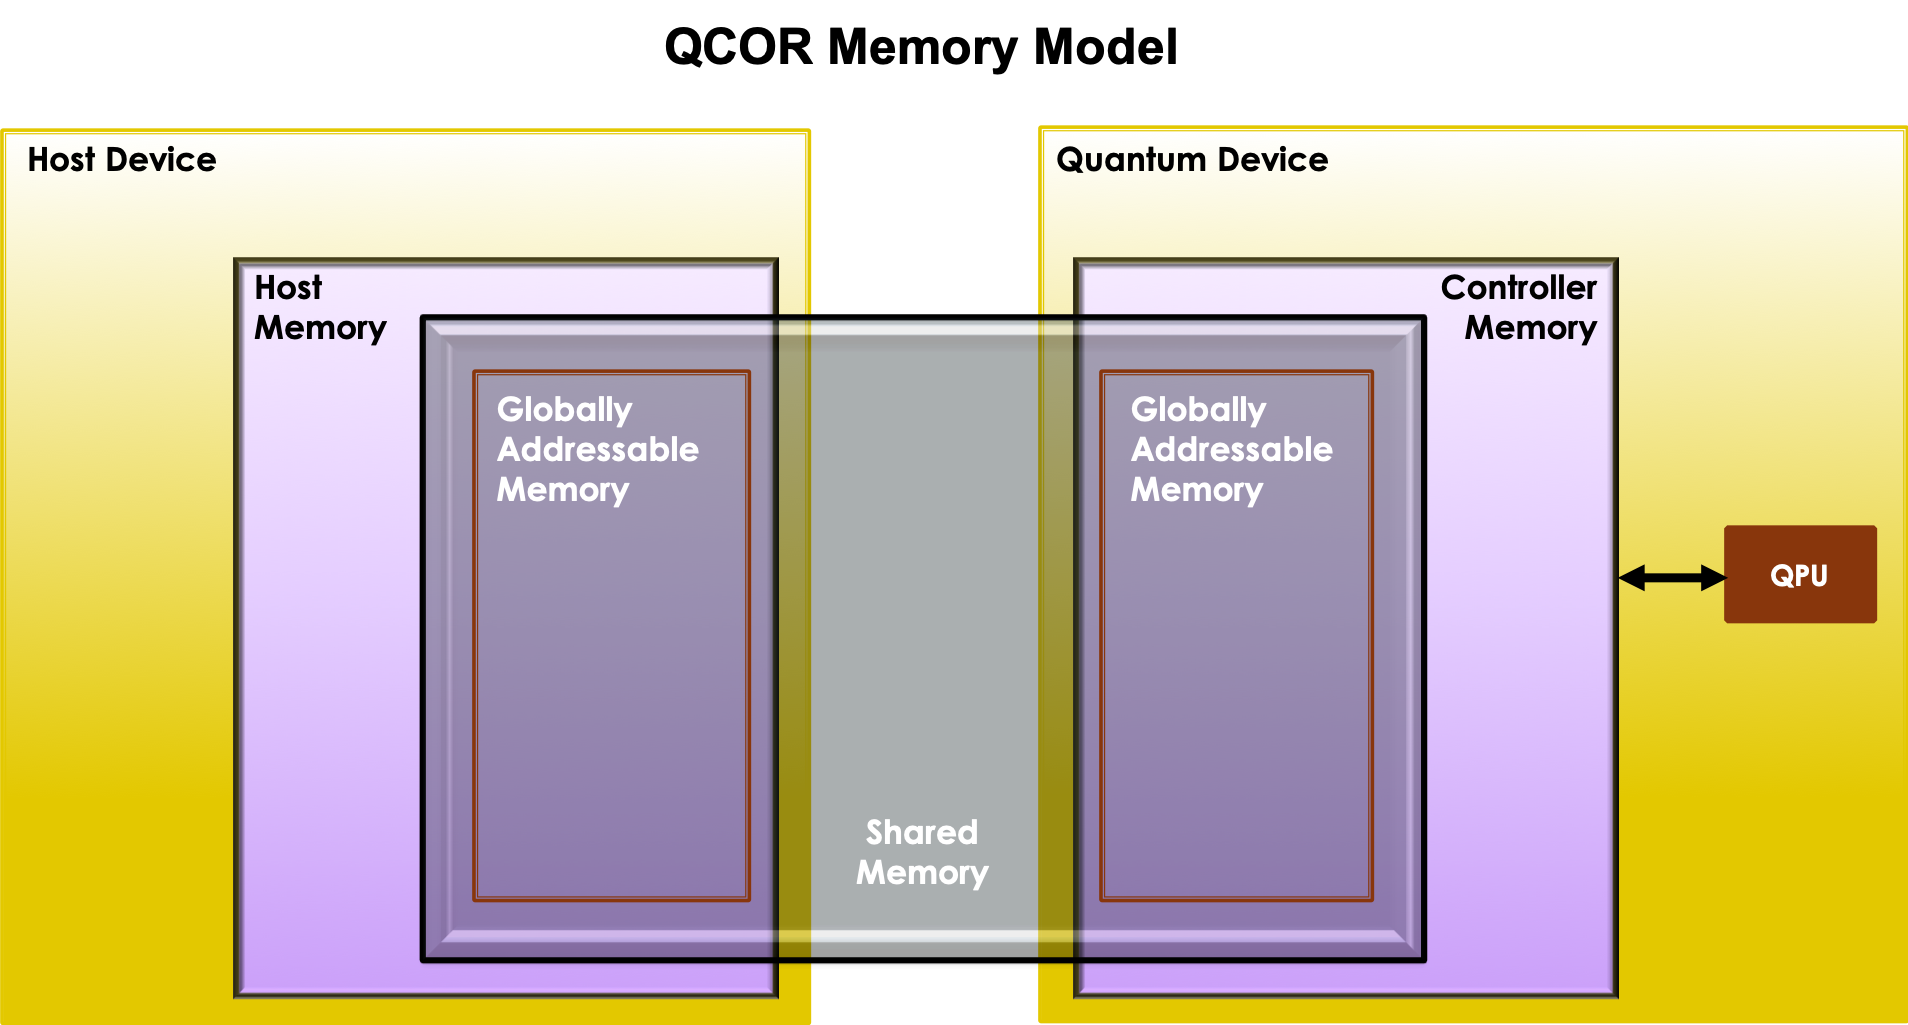
\includegraphics[height=3.5in,width=5.5in]{figures/Memory_Model_Illustration_v4.png}
  \caption{Diagram of the \qcor memory model}
  \label{fig:mem_model}
\end{figure*}
